\chapter{Vintergatans rörelse och struktur}
I detta kapitel så beskriver vi hur SALSA kan användas för att mäta Vintergatans
rörelse och struktur. Vi förklarar först hur vi kan mäta rotationskurvan, d.v.s.
rotationshastigheten för gas på olika avstånd från galaxens centrum.
Med hjälp av denna kunskap så gör vi sedan en karta över Vintergatan. 

\section{Vintergatans rotationskurva}
En rotationskurva är en funktion som beskriver rotationshastigheten $V$ för
galaxen vid olika avstånd $R$ från dess centrum, och betecknas vanligen $V(R)$. 
För att konstruera rotationskurvan från mätningar med SALSA så måste vi först
förstå hur den hastighet som vi observerar (genom Dopplereffekten) relaterar till
gasmolnens rörelse i galaxen. Anta att vi pekar vårt radioteleskop mot ett
gasmoln i galaxen, d.v.s. vi observerar längs den gröna linjen i figur \ref{fig:galgeom}.
\begin{figure}[ht]
\begin{center}
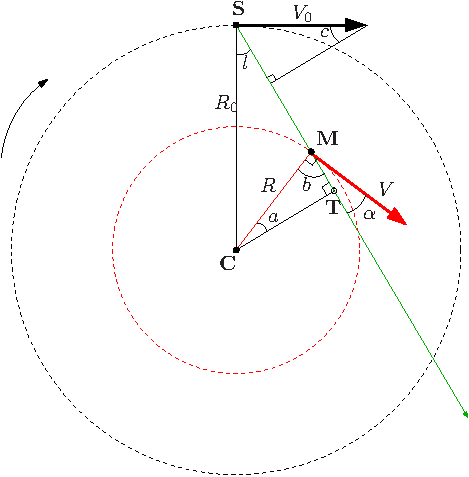
\includegraphics[width=8cm]{../figures/galgeom.pdf}
\end{center}
\caption{Vintergatans geometri. {\bf C} markerar galaxens centrum, {\bf S} är Solens position, 
	och {\bf M} är ett gasmoln som vi vill observera. Pilen vid sidan visar åt vilket håll
	galaxen roterar. Pilarna visar hastigheten för Solen ($V_0$) och för gasmolner ($V$).}
\label{fig:galgeom}
\end{figure}  
För framtida beräkningar så ger vi här en förklaring på de storheter som betecknas i figuren:
\begin{displaymath}
	\boxed{
\begin{array}{ll}
	V_0 	&\hbox{Solens hastighet runt galaxens centrum, d.v.s. 220 km/s}					\\
    R_0	&\hbox{Avståndet mellan Solen och galaxens centrum, d.v.s. 8.5 kpc} 					\\
l	&\hbox{Vald galaktisk longitud för vår observation}				\\
V	&\hbox{Hastigheten för gasmolnet}			\\
R	&\hbox{Avståndet mellan gasmolnet och galaxens centrum}		\\
\end{array}
}
\end{displaymath}

Det kan finnas många moln i denna riktning, men i denna härledning så bryr vi oss
bara om det moln som finns vid positionen $M$ i figur \ref{fig:galgeom}. Eftersom
både solen och molnet rör sig så mäter vi inte molnets hastighet direkt. Vi mäter
istället den relativa hastigheten, $V_r$, mellan oss och molnet, projicerad på
siktlinjen. Med vinklarna angivna i figure \ref{fig:galgeom} så kan vi 
skriva ner detta som  
\begin{equation}
V_r = V \cos\alpha - V_0 \sin c .
\label{eqn:vrel1}
\end{equation}
För att vi ska kunna använda denna ekvation så måste vi relatera vinklarna till
det galaktiska koordinatsystemet som vi beskrev i avsnitt \ref{sect:galcoords}.
Vi vet att summan av vinklarna i en övre rätvinkliga triangeln måste vara
180$^\circ$, vilket innebär att vi kan relatera vinkeln $c$ till den galaktiska
longituden $l$ på följande vis:
\begin{equation}
(90-l)+90+c=180 \quad \Rightarrow \quad c=l.
\label{eqn:c}
\end{equation}
Vi vill nu relatera även vinkeln $\alpha$ till longituden $l$. Vi ser att vinkeln 
mellan $V$ och $R$ är rät och kan skrivas som summan av $a$ och $\alpha$, d.v.s
$90^\circ = b + \alpha$. Vidare ser vi från triangeln {\bf CMT} att $b = 90^\circ - a$.
Sammantaget ger detta 
\begin{equation}
    90 = 90-a+\alpha \quad \Rightarrow \quad a = \alpha
\label{eqn:a}
\end{equation}
Från de två trianglarna {\bf CST} och {\bf CMT} ser vi att vi kan skriva
avståndet mellan galaxens centrum ({\bf C}) och tangentpunkten ({\bf T}) på två
olika sätt:
\begin{equation}
	{\rm\bf CT} = R_0\sin l = R \cos a \quad \Rightarrow \quad \cos a = \frac{R_0\sin l}{R}
\label{eqn:cosalpha}
\end{equation}
Genom att använda ekvationerna \ref{eqn:c}, \ref{eqn:a} och \ref{eqn:cosalpha}
så kan vi nu skriva om ekvation \ref{eqn:vrel1} såhär:
\begin{equation}
\boxed{V_r = V \frac{R_0}{R}\sin l - V_0 \sin l .}
\label{eqn:vrel2}
\end{equation}
Denna ekvation fungerar för alla longituder $l$. Men, att bara mäta $V_r$ för ett
givet $l$ är inte tillräckligt för att lösa denna ekvation för att få fram
både $V$ och $R$. Därför begränsar vi oss till de värden på $l$ som ligger
i den första kvadranten, och vi använder endast den maximala hastigheten
som vi mäter i varje spektrum. Hur kan detta göra vårt problem lättare att lösa?

Jo, i varje riktning så kan vi detektera strålning från flera gasmoln samtidigt.
Eftersom molnen rör sig med olika relativa hastigheter så ser vi flera komponenter
i vårt spektrum, se t.ex. figur \ref{fig:vmax}. 
\begin{figure}[ht]
\begin{center}
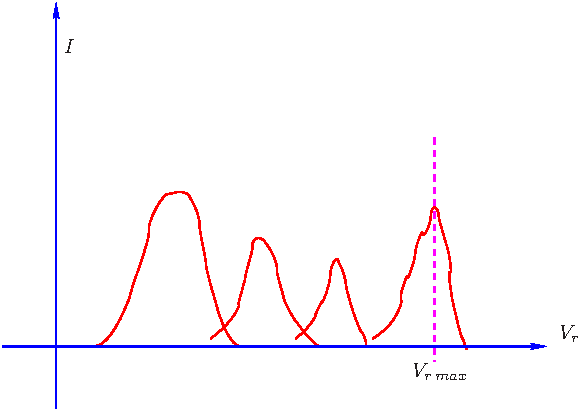
\includegraphics[width=10cm]{../figures/vmax.pdf}
\end{center}
\caption{Ett spektrum kan innehålla flera hastighetskomponenter, där varje
	komponent motsvarar ett moln med en viss relativ hastighet.}
\label{fig:vmax}
\end{figure}
Vi antar nu att moln som är längre bort från galaxens centrum än solen rör
sig med samma eller lägre hastighet som de moln närmare centrum, som vi 
väntar oss från normal Kepleriansk rörelse, (se Appendix. \ref{sect:kepler}).  
Detta innebär att komponenten med den {\bf högsta hastigheten}, $V_{\rm r,max}$, 
kommer från ett moln som befinner sig {\bf vid tangentpunkten } ({\bf T}), 
eftersom den maximala möjliga projicerade hastigheten uppmäts när
projiceringsvinkeln är 0 grader. För ett moln vid tangentpunkten
så ser vi från figur \ref{fig:galgeom} att molnets position ges av  
\begin{equation}
	R = R_0 \sin l.
	\label{eqn:rotR}
\end{equation}
Detta förenklar ekvation \ref{eqn:vrel2} så att vi nu, för ett moln vid tangentpunkten,
kan beräkna hastigheten som
\begin{equation}
V = V_{r,max} + V_0 \sin l .
\label{eqn:rotV}
\end{equation}
Vi kan alltså använda SALSA för att mäta $V_{\rm r,max}$ vid flera
olika $l$ i första kvadranten.  Genom att angända ekvationerna \ref{eqn:rotR} och 
\ref{eqn:rotV} så kan vi beräkna rotationskurvan $V(R)$. 
Det är rimligt att anta att rotationskurvan är densamma även i de andra tre
kvadranterna. 

\subsection{Att mäta rotationskurvan med SALSA}
\label{sect:SALSArot}
Efter att ha läst föregående avsnitt så bör du ha en ide om hur du kan mäta
rotationskurvan med SALSA. Instruktioner för hur du använder teleskopet finns i
dokumentet \emph{SALSA bruksanvisning} som du hittar på SALSA-hemsidan.
När du har observerat några spektra vid olika longituder, skriv ner den
maximala hastigheten för varje spektrum och rita upp rotationskurvan.  Det
enklaste sättet att få fram hastigheter är att använda pekaren direkt i
kontrollprogrammet och notera värdena från grafen, men du kan också använda mer
avancerade verktyg såsom Matlab. Instruktioner för hur du tar fram mätvärden
från dina spektra finns i dokumentet \emph{SALSA bruksanvisning}.  För att rita
upp rotationskurvan så kan du använda något program som du är van vid. Ett
enkelt och gratis program är det Excel-liknande \emph{LibreOffice Calc}, 
där du kan skriva in dina beräknade värden på V och R i ett kalkylark och sedan 
använda en {\tt xy-chart} för att rita upp rotationskurvan. Ditt resultat
bör likna figur \ref{fig:rotfinal}. Observera att rotationskurvan är nästan platt!
Detta är ett indirekt bevis för mörk materia i vår galax. Du kan också jämföra dina resultat
med resultaten i Appendix \ref{app:rotcurves}.

\begin{figure}[t]
\begin{center}
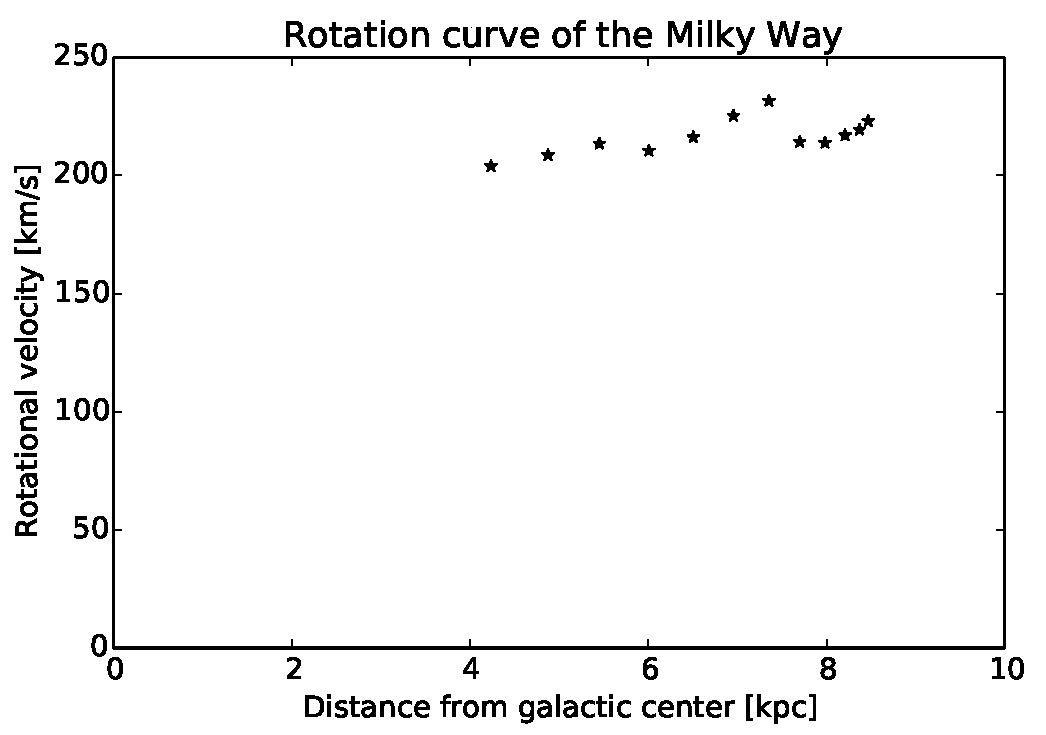
\includegraphics[width=0.7\textwidth]{../figures/SALSA_rotcurve.pdf}
\caption{En rotationskurva uppmätt med SALSA.}
\label{fig:rotfinal}
\end{center}
\end{figure}

\section{Kartläggning av Vintergatan}
\label{sect:map}
Nu vill vi ta reda på {\em var} gasen som vi observerat befinner sig.  Låt oss
därför återgå till ekvation \ref{eqn:vrel2}.  När vi tog fram rotationskurvan
så använde vi bara den högsta hastighetskomponenten i varje spektrum, och vi
antog att denna kommer från ett gasmoln vid tangentpunkten.  Detta antagande
gjorde det möjligt att lösa ekvation \ref{eqn:vrel2} i första kvadranten.  Nu
ska vi använda {\em alla hastighetskomponenter} som vi ser i varje spektrum,
och vi vill kunna observera i alla riktningar, inte bara i första kvadranten. 
Nu kan vi använda vår kunskap om rotationskurvan som vi tagit fram i avsnitt \ref{sect:SALSArot}.
Från vår uppmätta rotationskurva så antar vi nu att gasen i Vintergatan 
roterar {\em differentiellt}, d.v.s. att rotationshastigheten är konstant 
oavsett avstånd från centrum, och att den är samma som solens hastighet. Vi 
antar alltså att 
\begin{equation}
	V(R) = {\rm constant} = V_0.
\end{equation}
Med detta antagande så förenklas ekvation \ref{eqn:vrel2} till 
\begin{equation}
V_r = V_0\sin l \left( \frac{R_0}{R} -1 \right).
\end{equation}
Denna ekvation kan skrivas om till ett uttryck för molnets position $R$ 
som funktion av kända (eller observerbara som $V_r$) storheter och vi får 
\begin{equation}
\boxed{
R = \frac{R_0 V_0 \sin l}{V_0 \sin l + V_r}.
}
\label{eqn:Rmap}
\end{equation}
Nu vill vi skapa en karta över Vintergatan från de moln vi detekterat.
Från våra mätningar av den relativa hastigheten $V_r$ för varje moln
så kan vi beräkna avståndet mellan molnet och galaxens centrum. Eftersom
vi vet vilken riktning vi observerat (vår galaktiska longitud $l$) så 
kan vi få fram molnets position.

Det är viktigt att notera att om du observera i kvadrant II eller III, 
då finns det bara en möjlig position position för det strålande gasmolnet.
Men, om du observerar i kvadrant I eller IV, då kan det finnas {\em två möjliga positioners} 
som motsvarar $l$ or $R$: antingen närmare oss än tangentpunkten $T$ (d.v.s punkten
som markerats med {\bf M} i figur \ref{fig:galgeom}), eller längre bort, vid skärningen 
mellan linjen {\bf ST} och den inre cirkeln (se figur \ref{fig:galgeom}). 
{\bf Du kanske vill rita upp detta för att vara säker på att det stämmer.}

Denna tvetydighet för positioner kan också visas matematiskt. Låt $r$ vara 
avståndet från solen till molnet, d.v.s. avståndet mellan punkterna {\bf
S} och {\bf M} i  figur \ref{fig:galgeom}. Genom att använda cosinussatsen
på triangeln {\bf CSM} så får vi följande samband:
\begin{equation}
R^2 = R_0^2 + r^2 - 2 R_0 r \cos l.
\end{equation}
Detta är en andragradsekvation i $r$, som har två möjliga lösningar. Om vi
kallar dessa lösningar $r=r_{+}$ and $r=r_{-}$, så kan vi skriva ner ett 
allmänt uttryck för lösningarna som 
\begin{equation}
\boxed{
r_\pm = \pm \sqrt{R^2 - R_0^2 \sin^2 l} + R_0\cos l .
}
\label{eqn:rpm}
\end{equation}

I kvadranterna II och III så är $R$ alltid större än $R_0$ och $\cos l <0$,
vilket innebär att det finns en och endast en positiv lösning $r_+$. Den 
negativa lösningen är inte fysikaliskt intressant här (vi tittar inte genom jorden) 
och därför ignorerar vi den. 
I kvadranterna I och IV så kan det finnas två möjliga positiva lösningar.
I sådana fall så är det inte möjligt att bestämma vilken som är rätt utan att göra
fler observationer. För att reda ut vilken lösning som är sann så kan vi observera
igen mot samma galaktiska longitud men med en liten (några grader) vinkel
även i latitud. Om det tvetydiga molnet är långt bort så bör det nu försvinna. Om
molnet är nära så bör det fortfarande synas, även om vi observerar i en riktning
aningen ut från galaxens plan. Här kan du behöva prova dig fram för att hitta 
rätt latitud för att reda ut tvetydigheten. 

\subsection{Att konvertera från ($r,l$) till kartesiska koordinater} 
För att rita upp en karta så kan det vara opraktiskt att använda koordinaterna
$r$ (avståndet till molnet från solen) och $l$ (galaktisk longitud) för att beskriva
molnets position. Istället så är det oftast smidigare att konvertera till kartesiska koordinater
($x,y$). För att göra detta så måste vi relatera ($r, l$) till ($x, y$). 

Du är förmodligen bekant med \emph{polära koordinater}, som vanligen skrivs
\begin{equation}
\left\{ 
\begin{array}{l}
x=r \cos \theta \\
y=r \sin \theta \\
\end{array}
\right.
\label{eqn:polar}
\end{equation} 
där $r$ är avståndet från origo och $\theta$ är rotationsvinkeln, och $x$ and $y$ 
är kartesiska koordinater.  Dessa polära koordinater är väldigt lika våra koordinater
($r, l$), se figur \ref{fig:polar}.
\begin{figure}[ht]
\begin{center}
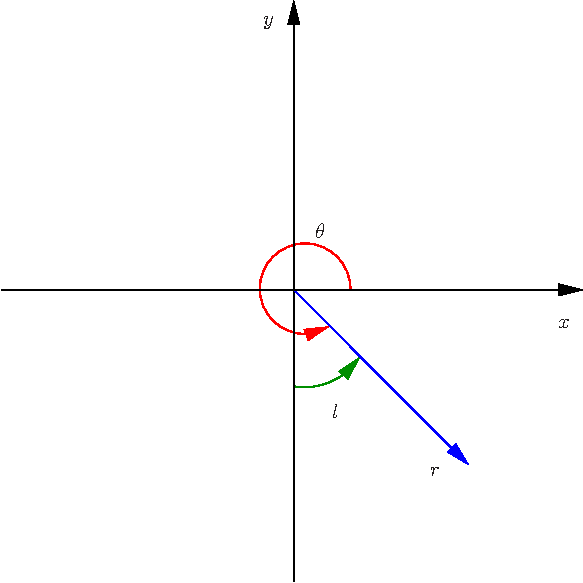
\includegraphics[width=0.5\textwidth]{../figures/coordinate.pdf}
\caption{Illustration av polära ($r$,$\theta$) och våra 
  ($r$,$l$) koordinater.}
\label{fig:polar}
\end{center}
\end{figure}
Vi ser att $\theta=270^\circ +l$, eller $\theta=l-90^\circ$. Detta innebär att vi kan konvertera våra positioner 
från ($r, l$) till kartesiska ($x, y$) genom ekvationerna
\begin{equation}
	\boxed{
\left\{ 
\begin{array}{l}
	x=r \cos (l-90^\circ) \\
	y=r \sin (l-90^\circ) \\
\end{array}
\right.}
\label{eqn:rpmtocart}
\end{equation} 
Detta format är vanligtvis det mest praktiska för att rita upp en karta. 

\subsection{Att göra en karta med SALSA}
\label{sect:SALSAmap}
Efter att ha läst föregående avsnitt så bör du ha en idé om hur du kan skapa
en karta från uppmätta hastigheter. Dessa mätningar görs på samma sätt 
som du gjorde i avsnitt \ref{sect:SALSArot}, men nu kan du mäta i alla kvadranter. 
Du kan nu också använda alla hastighetskomponenter i dina spektra.
Återigen så finns instruktioner för hur du använder teleskopet i dokumentet
\emph{SALSA bruksanvisning} som du hittar på SALSA-hemsidan.  När du har
observerat några spektra vid olika longituder, skriv ner den vilka hastigheter
som du ser i varje spektrum.
Det enklaste sättet att få fram hastigheter är att använda pekaren direkt i
kontrollprogrammet och notera värdena från grafen, men du kan också använda mer
avancerade verktyg såsom Matlab. Instruktioner för hur du tar fram mätvärden
från dina spektra finns i dokumentet \emph{SALSA bruksanvisning}.

När du har en lista över uppmätta hastigheter för flera longituder så kan du 
använda ekvation \ref{eqn:rpm} för att hitta positionen för molnen. Notera 
att observationer i kvadranterna I och IV kan behöva kompletteras med ytterligare
observationer för att reda ut eventuella tvetydigheter, se föregående avsnitt. 

För att göra din slutliga karta så kan du använda ditt favoritprogram. Återigen
så är ett enkelt och gratis program det Excel-liknande \emph{LibreOffice Calc},
där du kan skriva in dina beräknade värden ($x, y$) i ett kalkylark och sedan
använda en {\tt xy-chart} för att rita upp din karta. Din slutliga karta liknar
troligen figur \ref{fig:rotfinal}, men kartans exakta utseende kommer att bero
på de riktningar du observerat. Du kanske också vill jämföra med kartan om
omslaget till detta dokument. 

\begin{figure}[t]
\begin{center}
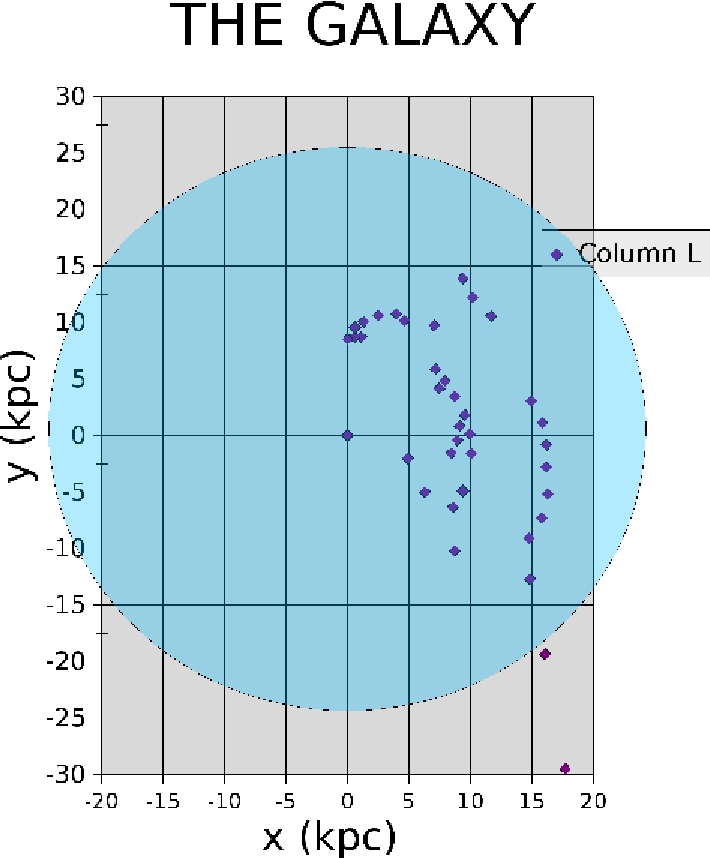
\includegraphics[width=0.6\textwidth]{../figures/galaxopenoffice1.pdf}
\caption{En karta över en del av Vintergatan gjord med data från SALSA. Kartan har 
	ritats med $xy$-chart in LibreOffice.  Vi kan tydligt se delar av spiralarmarna.
	Den blå cirkeln representrar galaxens utsträckning, med en diameter på ca 50~kpc.}
\label{fig:mapfinal}
\end{center}
\end{figure}
